\chapter{Processor architecture}

\section{Instruction Set architecture}

Instruction Set Architecture (ISA) defines the set of instructions and the registers on which they operate. From ISA-perspective all instructions are executed atomically, and their result is visible only after an execution is complete. ISA serves as an interface between software and actual hardware microarchitecture which implements the ISA. This abstraction allows software to reason about program behavior independently of the underlying microarchitectural implementation, which may use additional internal registers or buffers and update state at finer (cycle-level) granularity.


ISA defines binary format of instructions which are stored in memory and accessed by the processor through cache mechanisms. Often, fixed length instructions are used (for example, RISC architectures \TODO{reference}), while variable-length also exist (in CISC architectures \TODO{reference}). Processor is a cycled device that performs fetching instructions from memory and their subsequent execution, we call the microarchitectural state the state of all hardware registers of the processor. Unlike in ISA, states are defined at clock-cycle granularity, so an instruction may take several clock-cycles to finish. 

\TODO{rewrite}

\section{Processor Pipeline Stages}

Early processors executed instructions sequentially, completing one instruction before starting the next. This approach, known as non-pipelined or single-cycle execution, resulted in lower throughput because each instruction had to wait for the previous one to finish all processing steps. Modern processors, in contrast, employ pipelining, which overlaps the execution of multiple instructions by dividing the process into discrete stages. This significantly improves instruction throughput and overall performance by utilizing hardware resources more efficiently.

Although the exact decomposition into stages may vary across architectures, a typical processor pipeline consists of five fundamental stages. More advanced processors may further subdivide these stages to enhance performance.

We start by describing the fundamental pipeline stages and then introduce some optimizations such as superscalar pipelines, out-of-order execution and branch prediction.

\begin{enumerate}
    \item \textbf{Instruction Fetch (IF)}: The processor retrieves the next instruction from memory by the address from the program counter (PC). This access typically leverages the instruction cache to reduce latency.

    \item \textbf{Instruction Decode (ID)}: The fetched instruction, represented in binary format, is decoded to determine its type and the registers it operates on. During this stage, the required operands are read from the register file, and control signals are generated for subsequent pipeline stages depending on the instruction type.

    \item \textbf{Execute (EX)}: The instruction is executed in this stage. Arithmetic and logic operations are performed by dedicated \textit{functional units} (FUs), which are selected based on the decoded instruction type. For memory access or control flow instructions, the effective address or branch target is computed during this stage.

    \item \textbf{Memory Access (MEM)}: If the instruction involves a memory operation (load or store), this stage accesses the memory hierarchy to read or write data. Non-memory instructions are not affected by this stage.

    \item \textbf{Writeback (WB) or Commit (COM)}: The final stage writes the result of the instruction back to the register file, making it visible at the architectural (ISA) level. Only after this stage does the instruction's result become accessible to subsequent instructions.
\end{enumerate}


\section{Hazards}

Although pipelining significantly improves throughput, it is still susceptible to stalls -- situations where instruction progress is temporarily halted for one or more clock cycles. These stalls often result from dependencies and interactions among instructions within the program. 

In this section, we provide an overview of these hazards and later we discuss hardware mechanisms designed to mitigate their impact.

\subsection{Data Hazards}

Pipeline stalls can arise due to dependencies between instructions that access the same registers. There are three primary types of register dependencies:

\textbf{Read-After-Write (RAW)} dependencies, also known as true data dependencies, occur when an instruction requires a value that is produced by a preceding instruction. For example, in the expression $(1 + 2 * 3)$, the addition depends on the result of the multiplication, creating a RAW dependency between the two operations.

\textbf{Write-After-Write (WAW)} dependencies occur when two instructions write to the same register. To preserve program correctness, the writes must occur in program order, ensuring that the final value in the register corresponds to the last write.

\textbf{Write-After-Read (WAR)} dependencies arise when a younger instruction writes to a register that a previous instruction still needs to read. If the write occurs before the read, the earlier instruction may read an incorrect value.

RAW hazards are inherent to all architectures and must be handled to ensure correct execution. WAW and WAR hazards do not occur in simple in-order pipelines but must be addressed in more complex architectures such as out-of-order model, which will will be discussed in more details in the subsequent sections.

\subsection{Control Hazards}

Control hazards, also known as branch hazards, occur when the pipeline cannot determine the address of the next instruction to fetch due to the presence of a branch instruction. The outcome of the branch is typically resolved in the execute stage, leaving the pipeline uncertain about which instruction to fetch next.

To address this uncertainty, the pipeline introduces bubbles -- cycles in which no useful work is performed -- until the branch outcome is known. Figure \ref{fig:bubbles} illustrates a pipeline stall caused by a control hazard following a branch instruction.

\begin{figure}[H]
    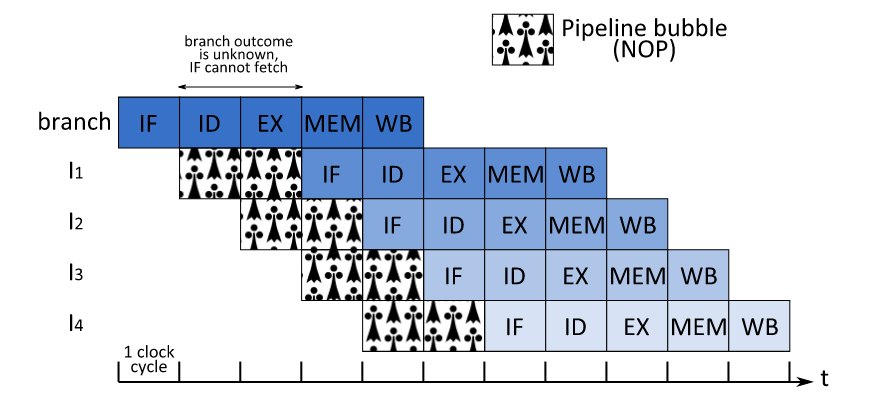
\includegraphics[width=\textwidth]{figures/pipeline-bubbles.png}
    \caption{Example of control hazard: the pipeline is stalled until branch finished the execution (from \cite{perais_increasing_2016})}
    \label{fig:bubbles}
\end{figure}

\section{Pipeline optimizations against data hazards}

\subsection{Bypass network}

In a conventional pipeline, operands for an instruction are read from the register file during the ID stage. Consequently, if instruction $B$ depends on the result of instruction $A$, $B$ must wait until $A$ completes its WB stage before it can proceed, introducing pipeline stalls. A bypass (or forwarding) network mitigates this delay by routing the result directly from the output of the EX or MEM stage to the input of the dependent instruction in the ID or EX stage, thereby reducing or eliminating the stall cycles caused by RAW dependencies. Figure \ref{fig:bypass-network} illustrates the effect of a bypass network on pipeline execution by comparing the 2 executions: without and with bypass network. As it can be observed, waiting for WB causes IF and ID stages to stall (noted with as \textit{if} and \textit{id} in lowercase).

\begin{figure}[H]
    \centering
    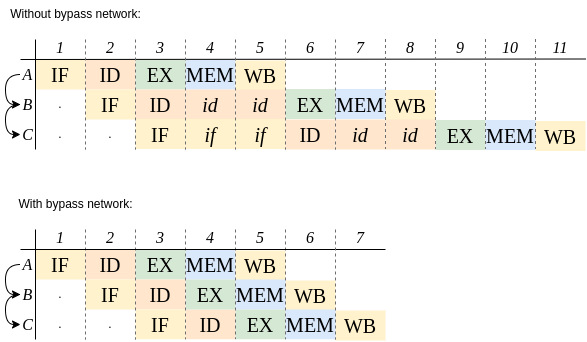
\includegraphics[width=0.7\textwidth]{figures/bypass network.png}
    \caption{Execution of the same 3 instructions with RAW dependencies (noted with arrow). Comparison of pipeline without and with bypass network.}
    \label{fig:bypass-network}
\end{figure}

\subsection{Superscalar Execution}

Superscalar execution allows the processor to fetch and execute multiple instructions at the same time. This means that some pipeline stages, such as instruction fetch (IF), decode (ID), and commit (COM), are duplicated to handle several instructions in parallel. For example, in Figure \ref{fig:superscalar}, six instructions are fetched as three pairs, which saves one clock cycle for each pair compared to a non-superscalar pipeline. If the instructions are independent, this can greatly improve performance. However, duplicating every pipeline stage is expensive. While it is relatively easy to duplicate IF, ID, and COM stages, it is much harder to duplicate the execution and memory access stages, so creating high superscalar-degree pipelines comes with a great hardware cost.

\begin{figure}[H]
    \centering
    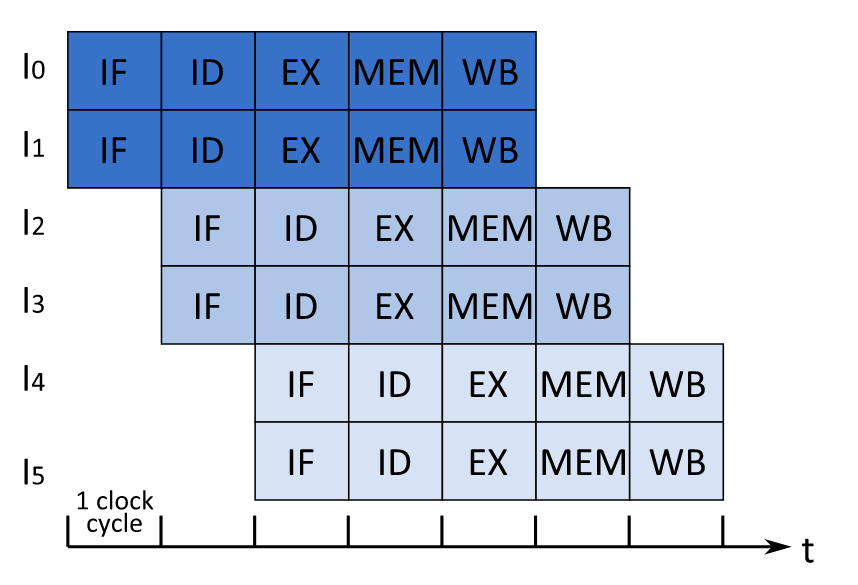
\includegraphics[width=0.7\textwidth]{figures/multiscalar-execution.png}
    \caption{Degree 2 superscalar pipeline: each pipeline stage can process up to two instructions per cycle, provided the instructions are independent.}
    \label{fig:superscalar}
\end{figure}

\subsection{Out-of-Order (OoO) Pipeline}
Out-of-Order (OoO) execution enables instructions to be processed based on data dependencies rather than strictly adhering to program order. While the architectural state (as defined by the ISA) must be updated in program order to preserve correctness, many instructions are independent and can be executed as soon as their operands are available. This parallelism improves resource utilization and overall throughput.

To support OoO execution while maintaining a consistent ISA-visible state, the processor pipeline is logically divided into in-order and out-of-order regions. The in-order region typically includes the instruction fetch (IF), decode (ID), and commit (COM) stages, while the out-of-order region encompasses execution and memory access stages. Instructions are fetched and decoded in program order, but may be executed and completed out of order, provided their dependencies are satisfied. Final commitment to the architectural state occurs in order, ensuring correctness.

Key hardware structures enable OoO execution:

\textbf{Reservation Stations (RS):} Each functional unit (FU) is associated with a reservation station, which buffers instructions waiting for execution. Once an instruction is decoded, it is dispatched to the appropriate RS based on its type. If the FU is busy or operands are not yet available, the instruction waits in the RS. The FU selects ready instructions from its RS for execution according to a scheduling policy.

\textbf{Reorder Buffer (ROB):} The ROB is a FIFO structure that tracks all instructions in flight between decode and commit. When an instruction enters the out-of-order region, it is allocated an entry in the ROB. Upon completion of execution, the instruction is marked as complete in the ROB. The commit stage retires instructions from the ROB in program order, updating the architectural state only when instructions at the head of the ROB have finished execution. This mechanism ensures that the ISA state is updated in the correct order, even though execution may have occurred out of order.

Figure \ref{fig:ooo-pipeline} shows the diagram of stage interconnections in processor. It represents the two optimizations discussed: superscalar and OoO execution.

\begin{figure}[H]
    \centering
    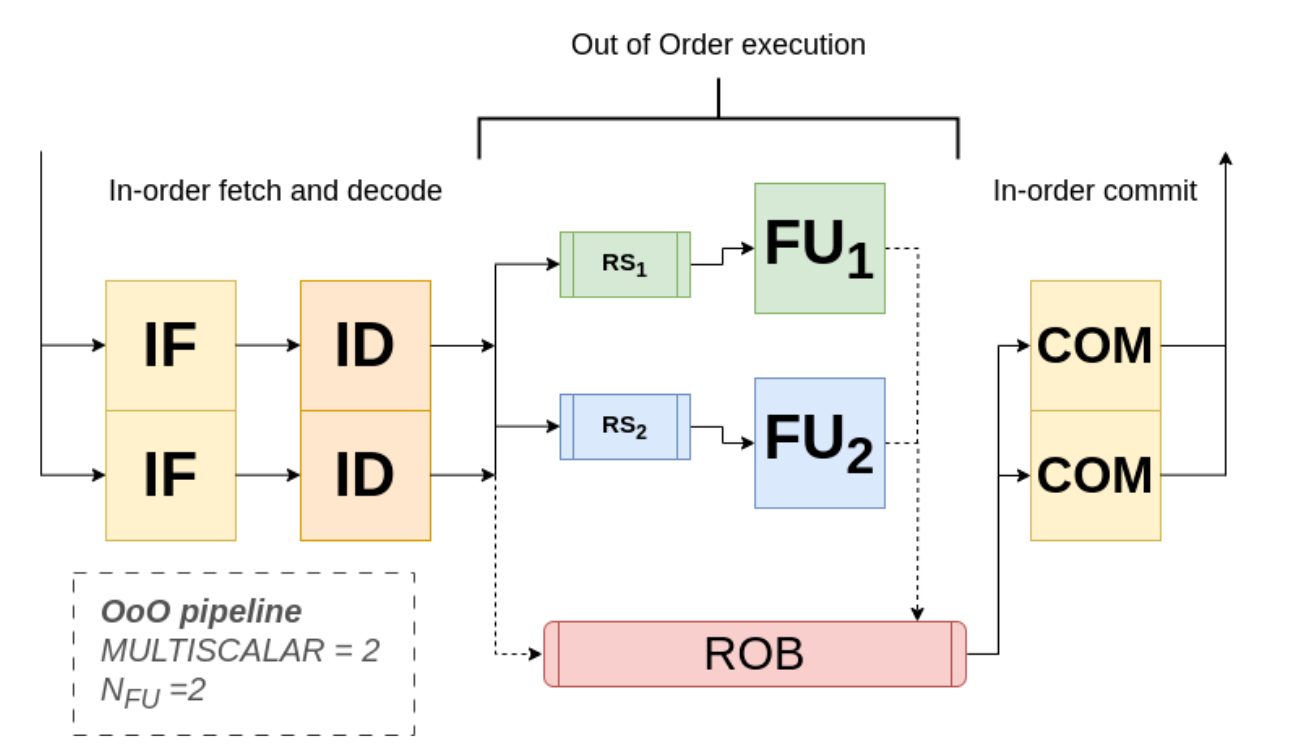
\includegraphics[width=0.6 \textwidth]{figures/ooo-pipeline.png}
    \caption{Out-of-Order superscalar pipeline diagram}
    \label{fig:ooo-pipeline}
\end{figure}

\section{Branch Prediction}

Thus far, we have discussed optimizations that address issues arising from data dependencies. Another critical aspect is the control flow of the program. When encountering a control divergence, such as a conditional branch, the processor cannot determine which instruction to fetch next until the branch condition is resolved.

In the processor pipeline, the Instruction Fetch (IF) stage is responsible for retrieving the next instruction. However, when a conditional jump instruction is encountered, the address of the subsequent instruction remains undefined until the branch outcome is computed. As a result, the pipeline must stall until the branch instruction completes execution.

To improve efficiency, modern processors employ branch prediction mechanisms to guess the likely outcome of a branch and speculatively fetch the corresponding instruction. These speculatively executed instructions are not committed to the architectural state until the branch decision is confirmed. If the prediction is incorrect, the speculative instructions are flushed from the pipeline (this is also called squashing), and execution resumes from the correct path.

Branch prediction by far is one of the most efficient optimizations in modern processors. By accurately predicting the outcome of branches, processors can keep their pipelines filled and minimize the number of stalls caused by control hazards. This leads to significant improvements in instruction throughput and overall performance, especially in workloads with frequent branching. The effectiveness of branch prediction is a key factor in the performance of superscalar and deeply pipelined architectures.

\subsection{Static Branch Predictors}

Static branch prediction utilizes information available at compile time to determine the likely outcome of each branch. Several strategies are commonly employed:

\textbf{Always Not Taken:} This strategy assumes that branches are never taken, and the processor continues fetching instructions sequentially. It generally yields lower prediction accuracy, particularly in programs with frequent branching.

\textbf{Always Taken:} Here, the predictor assumes that every branch will be taken. This approach often achieves higher accuracy than the "always not taken" strategy, especially in code with loops, where branches are typically taken except at loop exit.

\textbf{Backward Taken, Forward Not Taken (BTFNT):} This method predicts that backward branches (those targeting a lower address) are taken, while forward branches are not taken. BTFNT is particularly effective for loop constructs, as loop-closing branches are usually backward and taken, whereas forward branches often correspond to loop exits or conditional statements.

\subsection{Dynamic Branch Predictors}

Dynamic Branch Predictors rely on information retrieved from execution and are usually based on previous branch outcomes. The usage of dynamic branch predictors requires additional hardware components which are discussed below.

\textbf{Pattern History Table (PHT)} is used to store information about each branch. It can be a bit denoting whether the branch was taken last time, or a more complex data. PHT is usually indexed by the lower bits of branch instruction address.

\textbf{Branch Target Buffer (BTB)} stores the destinations of previously computed branch. When starting speculative execution, values from BTB are used.

\textbf{Return Stack Buffer (RSB)} is used to predict the outcome of \textit{ret} instructions.

\subsubsection{One-Bit Predictor}

The one-bit predictor is the simplest type of dynamic branch predictor. It uses PHT indexed by lower bits of address where one-bit value encodes the last branch outcome. Such a simple predictor is efficient when branch decision is not often changed throughout execution. For example, loop conditions are mispredicted only twice by this type of predictor: on the first and the last iterations of the loop.

However, more complex patterns diminish the efficiency of one-bit predictor. For instance, if branch outcome changes each time, the predictor accuracy is zero.

\subsubsection{Two-Bit Predictor}

The two-bit predictor uses the same idea of PHT-indexing, but instead of storing just the outcome of previous branch, it has 4-state automaton encoded by 2 bits. The states are STRONG-TAKEN, WEAK-TAKEN, WEAK-NTAKEN and STRONG-NTAKEN. Figure \ref{fig:two-bit-counter} shows the transitions between the states.

\begin{figure}[H]
    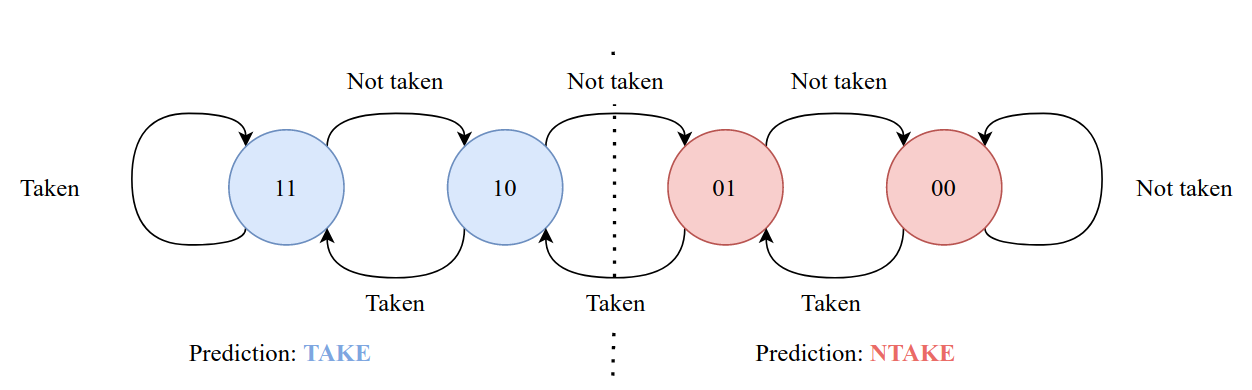
\includegraphics[width=\textwidth]{figures/two-bit-counter.png}
    \caption{Two-bit predictor state machine (from \cite{mahling_reverse_2023})}
    \label{fig:two-bit-counter}
\end{figure}

The two-bit predictor outperforms the one-bit predictor because it requires two consecutive mispredictions before changing its prediction direction. This makes it more resilient to occasional anomalies, where a one-bit predictor would immediately flip its prediction after a single misprediction. As a result, the two-bit predictor achieves higher accuracy, especially in scenarios with repetitive branch behavior.

